Este capítulo apresentará o método proposto por este trabalho para o projeto de prótese ativa baseada em sensores e aprendizado de máquina.

\section{\todo{Corrigir este título}A prótese}
\label{sec:metodo_protese}
\todo[inline]{Explicar o funcionamento geral, relacionando à big picture}
\label{sec:metodo_geral}
\begin{figure}[h]
	\caption{\label{fig:big_picture}Visão geral do protótipo}
	\begin{center}
	    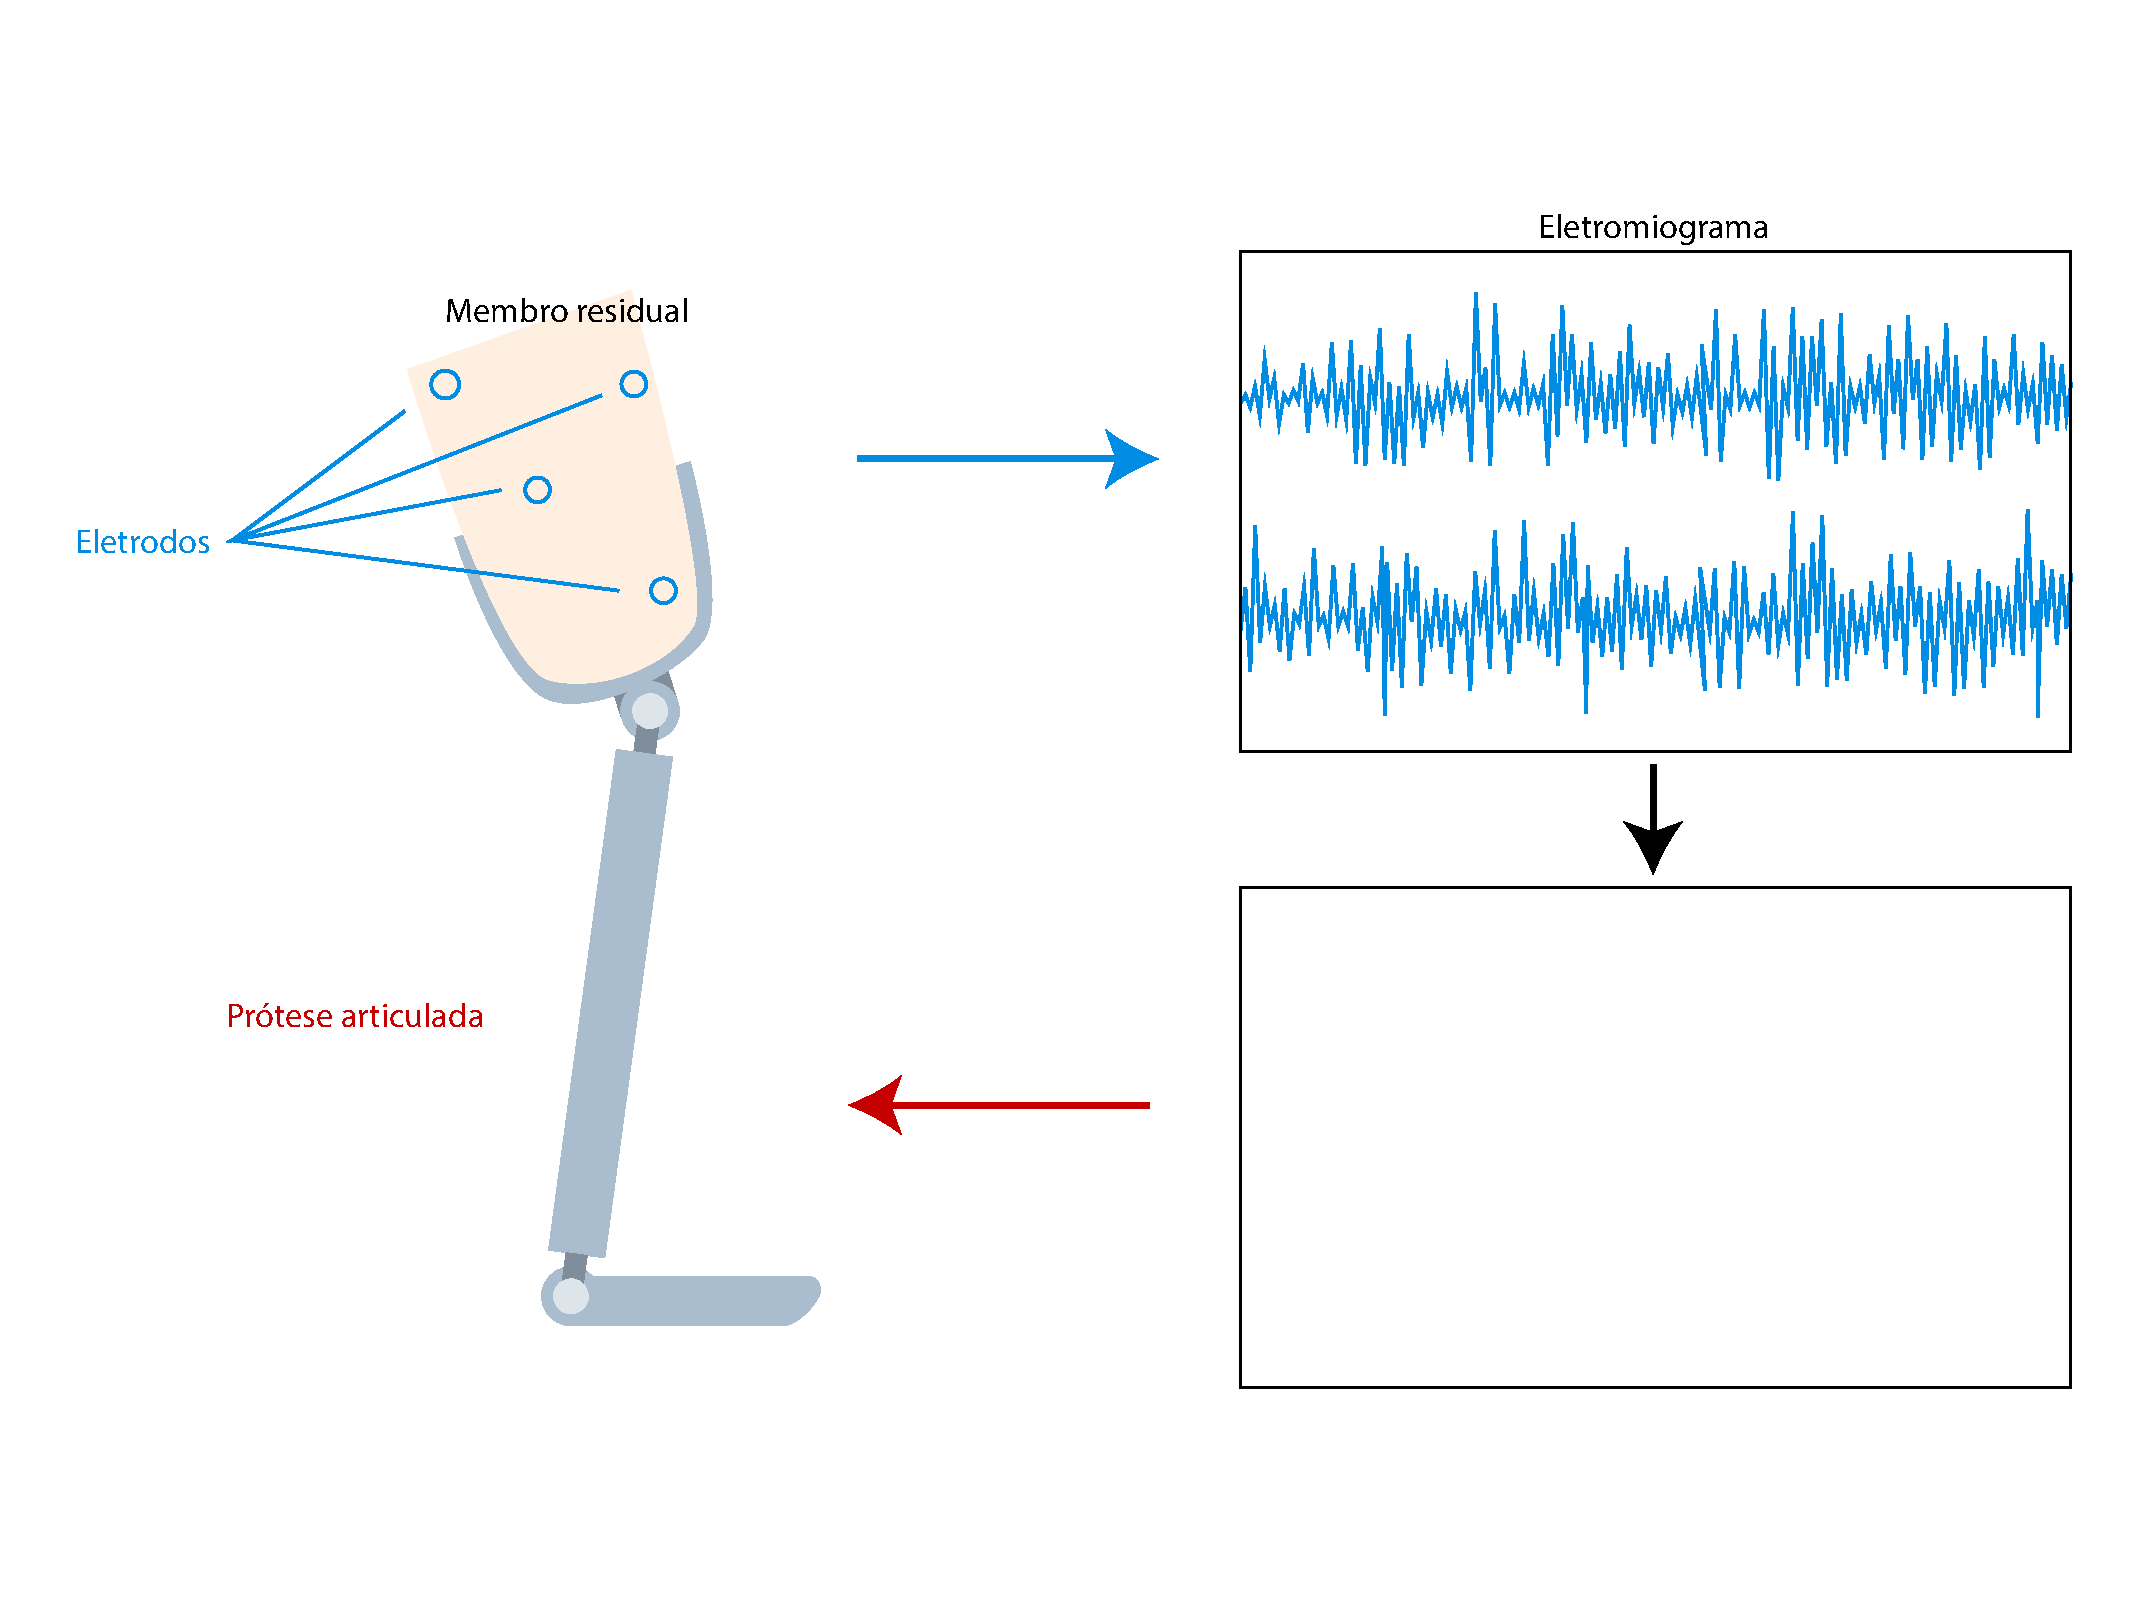
\includegraphics[width=0.8\textwidth]{resources/big_picture}
	\end{center}
	\legend{Fonte: Elaborada pelo autor}
\end{figure}

\todo[inline,color=lightgray]{Projeto e prototipação de uma prótese robótica para pé\\Como criar;\\Onde vão estar os sensores, materiais de baixo custo, próteses 3D;\\O que a prótese gera?; Atuadores; Gerar perguntas.}
\todo[inline]{Como vai ser a fonte de energia da prótese?}

\section{Coleta de dados e classificação}
\todo[inline,color=lightgray]{Coleta de dados dos sensores -- que sensores, que dados. Por que os dados são importantes: usar técnicas pra prever e identificar dados (Seção explicando da coleta, uma seção pra cada tipo de classificação)}

\todo[inline]{\textbf{Nova seção?}}
\todo[inline,color=lightgray]{Geração de movimentos: a partir dos dados coletados. Os atuadores vão tentar identificar os ambientes. Na escada, o motor vai fazer tal coisa, etc. Na rampa, etc.}

\todo[inline]{\textbf{Nova seção?}}
\todo[inline,color=lightgray]{Analisar saúde do caminhar. Se não tá caminhando torto. Gerar estatísticas do uso da prótese. (Os dados estão fazendo a pessoa puxar mais pra uma perna)}